\documentclass[10pt,t,english,aspectratio=1610]{beamer}
\usepackage{fontawesome}
\usepackage{graphicx}
\usepackage{array}
\usepackage[normalem]{ulem}
\usepackage{amsfonts,amsmath,amssymb,bm,bbm}
\usepackage{mathrsfs}
% NOTE: sgame is intentionally NOT used -- its `game` environment is
% incompatible with the `array` package (required by colortbl/makecell/multirow)
% and errors with "Missing # inserted in alignment preamble". We use the modern
% TikZ-based `xgames` package instead (loaded after TikZ below).
\usepackage{graphicx,pstricks}
\usepackage{xcolor}
\usepackage{colortbl}
\usepackage{makecell}
\usepackage{tikz,tikzsymbols,gnuplottex}
\usetikzlibrary{decorations.pathreplacing,shapes,positioning,arrows.meta,fit,backgrounds,calc}

% --- xgames: TikZ-based game-theory typesetting (matrixgame, gametree,
% beliefspace, automaton). Not on CTAN; xgames.sty + fikz.sty are vendored at
% the repo root. CC BY-SA 4.0 (xgames) / GPL-3.0 (fikz), (c) Benjamin Bernard.
\usepackage{xgames}

% Custom command for shading rows in a matrixgame
% ---------------------------------------------------------------------------
% \shaderow[<fill options>]{<row>}{<first column>}{<last column>}
% Call this inside the matrixgame, after \payoffmatrix
% Can wrap in a \foreach to shade multiple regions
% Example: \foreach \i in {1,...,5}{ \shaderow[green!50!black]{\i}{\i}{5} }
\newcommand{\shaderow}[4][red!60]{%
  \ifnum#3=1\relax\def\xl{0}\else\pgfmathsetmacro{\xl}{\pmtwi[#3-1]}\fi
  \ifnum#2=1\relax\def\yt{0}\else\pgfmathsetmacro{\yt}{\pmthi[#2-1]}\fi
  \pgfmathsetmacro{\xr}{\pmtwi[#4]}%
  \pgfmathsetmacro{\yb}{\pmthi[#2]}%
  \fill[opacity=0.18, #1] ($(pmt1-tl)+(\xl,-\yt)$) rectangle ($(pmt1-tl)+(\xr,-\yb)$);%
}

\usepackage[english]{babel}
\usepackage[utf8]{inputenc}
\usepackage{appendixnumberbeamer}
\usepackage{datetime2}
\usepackage{booktabs}
\usepackage{setspace}
\usepackage{rotating}
\usepackage{multirow}
\usepackage{listings}

\usepackage{natbib}
\bibliographystyle{unsrtnat}
\renewcommand{\bibfont}{\footnotesize}
\renewcommand{\bibsection}{\vspace{-1em}}

%\usepackage{matlab-prettifier} % For enhanced MATLAB highlighting
\lstset{
    language=matlab,
    % Other options for styling (optional)
    basicstyle=\ttfamily\footnotesize, % Font style
    keywordstyle=\color{blue}, % Keyword color
    commentstyle=\color{green!50!black}, % Comment color
    stringstyle=\color{red!70!black}, % String color
    numbers=left, % Line numbers on the left
    numberstyle=\tiny\color{gray}, % Style for line numbers
    frame=single, % Frame around the listing
    breaklines=true, % Allow line breaking
    captionpos=b, % Caption at the bottom
    tabsize=4 % Tab size
}

% ------------------------------------------------------------------------------
% Use the beautiful metropolis beamer template
% ------------------------------------------------------------------------------
\usepackage[T1]{fontenc}
\usepackage[utf8]{inputenc}
\usepackage{fontawesome}
\usepackage{FiraSans} 
\mode<presentation>
{
  \usetheme[progressbar=foot,background=light]{metropolis} 
  \usecolortheme{default} % or try albatross, beaver, crane, ...
  \usefonttheme{default}  % or try default, serif, structurebold, ...
  \setbeamertemplate{navigation symbols}{}
  \setbeamertemplate{caption}[numbered]
  %\setbeamertemplate{frame footer}{My custom footer}
  \makeatletter
    \setbeamertemplate{frametitle continuation}{}
  \makeatother
} 
\addtobeamertemplate{frametitle continuation}{}{%
  \setbeamertemplate{frametitle continuation}{}%
}
\setbeamertemplate{frametitle continuation}{}

\newenvironment{stepenumerate}{\begin{enumerate}[<+->]}{\end{enumerate}}
\newenvironment{stepitemize}{\begin{itemize}[<+->]}{\end{itemize} }
\newenvironment{stepenumeratewithalert}{\begin{enumerate}[<+-| alert@+>]}{\end{enumerate}}
\newenvironment{stepitemizewithalert}{\begin{itemize}[<+-| alert@+>]}{\end{itemize} }

\newtheorem{question}{Question}
\newtheorem{claim}{Claim}
\newtheorem{proposition}{Proposition}
\newtheorem{remark}{Remark}
\newtheorem{conjecture}{Conjecture}

\definecolor{metrop}{RGB}{29, 44, 44}
\colorlet{GrayLight}{black!15}
\colorlet{GrayMedium}{black!30}
\colorlet{ForestGreen}{green!60!black}

\newenvironment{transitionframe}{
  \setbeamercolor{background canvas}{bg=black!80}
  \begin{frame}}{
    \end{frame}
}

\newcommand{\bsk}{

\bigskip

}

\newcommand{\pd}{\partial}
\newcommand{\RR}{\mathbb{R}}

\newcommand*\hugme[1]{\tikz[baseline=(char.base)]{\node[shape=ellipse,draw,inner sep=0pt] (char) {#1};}}

\newcounter{saveenumi}
\newcommand{\seti}{\setcounter{saveenumi}{\value{enumi}}}
\newcommand{\conti}{\setcounter{enumi}{\value{saveenumi}}}
\resetcounteronoverlays{saveenumi}



\newcommand\dotprod[2]{\langle #1 , #2 \rangle}
\newcommand{\ft}[1]{\widehat #1}
\newcommand{\qabove}[1]{\overset{\text{\large \textbf ?}}{#1}}
\newcommand{\eqae}{\overset{\text{a.e.}}{=}}
\newcommand{\calp}{\mathcal{P}}
\newcommand{\calg}{\mathcal{G}}
\newcommand{\calb}{\mathcal{B}}
\newcommand{\textd}{\text{d}}
\newcommand{\bbr}{\mathbb{R}}
\newcommand{\binm}{\mathbin{M}}
\newcommand{\binc}{\mathbin{C}}
\newcommand{\binb}{\mathbin{B}}
\newcommand{\calc}{\mathcal{C}}
\newcommand{\calh}{\mathcal{H}}
\newcommand{\bfone}{\mathbf{1}}
\newcommand{\bbe}{\mathbb{E}}
\newcommand{\bfle}{\mathbf{e}}
\newcommand{\calf}{\mathcal{F}}
\newcommand{\cala}{\mathcal{A}}
\newcommand{\cale}{\mathcal{E}}
\newcommand{\bbn}{\mathbb{N}}
\newcommand{\cantor}{\calc}
\newcommand{\calY}{\mathcal{Y}}
\newcommand{\textb}{\text{B}}
\newcommand{\calm}{\mathcal{M}}
\newcommand{\bint}{\mathbin{T}}
\newcommand{\ep}{\epsilon}
\newcommand{\bbq}{\mathbb{Q}}
\newcommand{\bbp}{\mathbb{P}}
\newcommand{\cals}{\mathcal{S}}
\newcommand{\emptysequence}{e}
\newcommand{\bbz}{\mathbb{Z}}
\newcommand{\fraka}{\frak{A}}
\newcommand{\frakb}{\frak{B}}
\newcommand{\length}{\text{length}}
\newcommand{\bfn}{\mathbf{N}}
\newcommand{\support}{\text{support}}
\DeclareMathOperator*{\argmax}{arg\,max}
\newcommand{\dom}{\mbox{dom}}
\def\ut{\underline t}
\def\um{\underline m}
\def\PP{\mathbb{P}}
\def\EE{\mathbb{E}}
\def\RR{\mathbb{R}}

% Title page info
\title[Mixed Strategies]{Chapter 6: Mixed Strategies}
\author[ECON 5001]{ECON 5001\\Prof. Paul J. Healy\\Based on: \textit{Game Theory} by Giacomo Bonanno} \color{metrop}
\institute[OSU]{}
\date[]{\vfill {\tiny Updated \today\ at\ \DTMcurrenttime}}

% ---------------------------------------------------------------------
% SCOPE AND NOTATION
%   Same as deck 07: u(o) = outcome utility, U(L) = expected utility.
%   pi_i(s) = payoff at a pure profile; Pi_i(sigma) = expected payoff at a
%   mixed profile (Bonanno's notation for the second).
%   Section 6.1's lottery-valued outcome function f: S -> L(O) is NOT
%   taught. One slide says a cell can hold a lottery and that we then use
%   its expected utility as the payoff. Nothing later depends on more.
%   Section 6.4's correlated-beliefs discussion (3+ players, Aumann) is a
%   footnote only.
%
% ANSWERS (all checked by support enumeration; every NE below is unique)
%   Two-point conversion, payoffs = % chance OSU scores (Michigan: 100 - that)
%       Run:  40 vs Stop Run, 80 vs Stop Pass
%       Pass: 90 vs Stop Run, 30 vs Stop Pass
%     No pure NE. OSU Run 3/5, Michigan Stop Run 1/2. OSU scores 60%.
%     Pi_OSU(Run, q) = 80 - 40q ; Pi_OSU(Pass, q) = 30 + 60q
%     Practice profile OSU (1/2,1/2), Michigan (0.8, 0.2):
%       cell probs .4/.1/.4/.1 ; Pi_OSU = 16+8+36+3 = 63 ; Pi_UM = 37
%       vs q = 0.8: Run 48, Pass 78 -> OSU should Pass for sure
%   Goeree-Holt matching pennies (cents)
%     Symmetric: NE 1/2, 1/2.  Asymmetric (320): Row Top 1/2 (!),
%     Column Left 1/8. Lab: Top 96%, Left 16%.
%   Sunday Morning (deck 03, Story A payoffs, now read as cardinal)
%     Pure NE (B,B) = (4,3) and (H,H) = (3,4). Mixed: Alex B 1/2,
%     Blair B 1/4, payoffs (2.5, 2.5). Both prefer either pure NE.
%     If Alex's 4 becomes 10: Blair's mix becomes B 1/10. Alex's stays 1/2.
%   Bonanno Fig 6.7: A=3q, B=3-3q, C=2 (q = Pr D)
%     BR1: B if q<1/3, C if 1/3<q<2/3, A if q>2/3
%     NE: P1 (0, 1/3, 2/3), P2 (1/3, 2/3)
%   Deck 04's "never a best reply" M (3,3,3) vs U (4,2,4), D (0,4,0)
%     vs (L .4, C .6, R 0): U 2.8, M 3, D 2.4 -> M is the unique BR
%     M is a BR exactly when Pr(C) is in [1/2, 3/4], so not dominated
%   Bonanno Fig 6.9: B (1,1) dominated by 1/3 A + 2/3 C = (4/3, 4/3)
%   Bonanno Fig 6.10: C out (by 1/2 A + 1/2 B), F out (by 1/2 D + 1/2 E),
%     B out (by A), E out (by D). Rationalizable: A and D.
% ---------------------------------------------------------------------

% Lottery over {Score, Fail} in a cell of the two-point table, with a strut
% for row height (arraystretch would also stretch the pmatrix)
\newcommand{\lot}[2]{\rule[-0.22in]{0pt}{0.55in}$\begin{pmatrix} \text{Score} & \text{Fail} \\ #1 & #2\end{pmatrix}$}

\begin{document}

\frame{\maketitle}

\begin{frame}{Where We Left Off}
Chapter 2: some games have \textbf{no} Nash equilibrium
\begin{itemize}
    \item Matching Pennies, penalty kicks, play-calling...
    \item Being predictable gets you exploited
\end{itemize}
\bsk
Chapter 5: \textbf{expected utility} ranks lotteries
\begin{itemize}
    \item $u(o)$: outcome utility \qquad $U(L)$: expected utility
\end{itemize}
$$
    U(L) = \sum_i p_i\,u(o_i)
$$
\vfill
Our goal:
\begin{enumerate}
    \item Let players \textbf{randomize}
    \item Use expected utility to evaluate strategies in the face of a random opponent
    \item Redefine equilibria to include random play
    \begin{itemize}
        \item Show that, with this definition, it always exists
    \end{itemize}
\end{enumerate}
\vspace{-0.4in}
\end{frame}

% ==============================================================
% MOBLAB --- PLAY FIRST
% ==============================================================

% ---- MobLab run: Matrix: Instructor Specified ------------------------
% Goeree & Holt (2001) matching pennies, payoffs in cents. Two one-shot
% rounds, re-paired between rounds:
%   Round 1 (symmetric):  T: (80,40) (40,80)   B: (40,80) (80,40)
%   Round 2 (asymmetric): T: (320,40) (40,80)  B: (40,80) (80,40)
% Play BEFORE mixed strategies are defined. Results come back in
% "Back to MobLab".
% ---------------------------------------------------------------------
\begin{frame}{MobLab: ``Matrix: Instructor Specified'' $\times 2$}
\begin{itemize}
    \item MobLab time!
    \item You'll be paired with someone. Row player or Column player
    \item Two rounds, new partner each round. Each round played once
\end{itemize}
\bsk
\begin{columns}[T]
\begin{column}{0.48\textwidth}
\centering
\textbf{Round 1}\\[4pt]
\begin{matrixgame}[top={Left, Right}, left={Top, Bottom}, player names={Row, Column}]
  \payoffmatrix{80,40 & 40,80 \\ 40,80 & 80,40}
\end{matrixgame}
\end{column}
\begin{column}{0.48\textwidth}
\centering
\textbf{Round 2}\\[4pt]
\begin{matrixgame}[top={Left, Right}, left={Top, Bottom}, player names={Row, Column}]
  \payoffmatrix{\textbf{320},40 & 40,80 \\ 40,80 & 80,40}
\end{matrixgame}
\end{column}
\end{columns}
\vfill
\centering
\only<1>{Feel free to talk! And play it the way you'd actually play it.}
\only<2->{Who should respond to 320? Row? Column? Both?\\}
\only<3>{Paradoxical prediction: \textbf{Column} responds, \textbf{not} row}
\vspace{-0.3in}
\end{frame}

% \begin{frame}{MobLab Results}
% \vspace{0.5in}
% \centering
% \renewcommand{\arraystretch}{2}
% \begin{tabular}{l|c|c|}
% \cline{2-3}
%  & \% of Rows playing Top & \% of Columns playing Left \\
% \hline
% \multicolumn{1}{|l|}{Round 1} & \hspace{1in} & \hspace{1in} \\
% \hline
% \multicolumn{1}{|l|}{Round 2} & & \\
% \hline
% \end{tabular}
% \end{frame}

% ==============================================================
% 6.1 STRATEGIC-FORM GAMES, REVISITED
% ==============================================================

\begin{frame}[standout]
Strategic-Form Games With Randomness
\end{frame}

\begin{frame}{Strategic-Form Games}
Same as Chapter 2:
\bsk
\centering
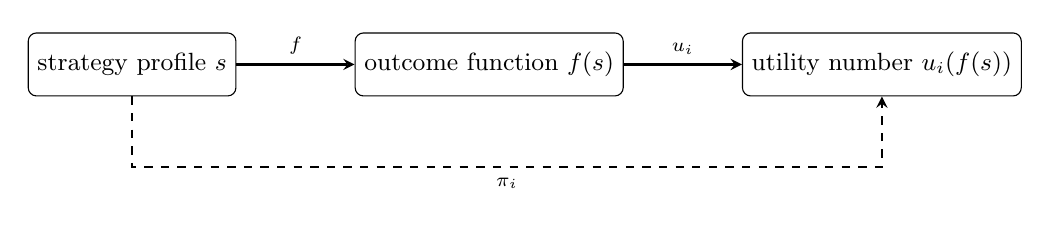
\begin{tikzpicture}[>=stealth, node distance=1.0cm,
   box/.style={draw, rounded corners=3pt, minimum height=0.8cm, minimum width=2.4cm, font=\small}]
  \node[box] (s) {strategy profile $s$};
  \node[box, right=1.5cm of s] (o) {outcome function $f(s)$};
  \node[box, right=1.5cm of o] (u) {utility number $u_i(f(s))$};
  \draw[->, thick] (s) -- node[above, font=\scriptsize] {$f$} (o);
  \draw[->, thick] (o) -- node[above, font=\scriptsize] {$u_i$} (u);
  \draw[->, thick, dashed] (s.south) -- ++(0,-0.9) -| node[below, pos=0.25, font=\scriptsize] {$\pi_i$} (u.south);
\end{tikzpicture}
\bsk
\raggedright
\vspace{0.2in}
\begin{itemize}
    \item Payoff $\pi_i(s)$ gives $i$'s utility for the outcome generated by $s$
    \begin{itemize}
        \item No need to specify outcomes, just payoffs
    \end{itemize}
    \item Utility numbers are \textbf{expected utility values}, like little $u(o_i)$
    \begin{itemize}
        \item Remember: only linear rescaling is allowed
    \end{itemize}
    \item Bonanno: ``games with cardinal payoffs''
\end{itemize}
\end{frame}

\begin{frame}{How To Evaluate Randomness?}
\begin{center}
\begin{matrixgame}[top={Rock,Paper,Scissors}, left={Rock,Paper,Scissors}]
  \payoffmatrix{Draw & Lose & Win \\ Win & Draw & Lose \\ Lose & Win & Draw}
\end{matrixgame}\\
P1's outcome shown
\end{center}
\bsk
\begin{itemize}
    \item<2-> Player 1: Win $\succ$ Draw $\succ$ Lose
    \item<3-> Let's try: $u(Win)=1$, $u(Draw)=0$, $u(Lose)=-1$
    \item<4-> And suppose your opponent is playing each strategy with $1/3$ chance
\end{itemize}
\end{frame}

\begin{frame}{How To Evaluate Randomness?}
\begin{center}
\begin{matrixgame}[top={R ($1/3$),P ($1/3$),S ($1/3$)}, left={Rock,Paper,Scissors}]
  \payoffmatrix{0 & -1 & 1 \\ 1 & 0 & -1 \\ -1 & 1 & 0}
\end{matrixgame}\\
P1's outcome utility ($u(o)$) shown
\end{center}
\bsk
Use expected utility to evaluate strategies:
\begin{itemize}
    \item $U(\text{Rock}) = (1/3)\cdot 0+(1/3)\cdot(-1)+(1/3)\cdot 1 = 0$
    \item $U(\text{Paper}) = (1/3)\cdot 1 + (1/3)\cdot 0 + (1/3)\cdot(-1) = 0 $
    \item $U(\text{Scissors}) = (1/3)\cdot (-1)+(1/3)\cdot 1+(1/3)\cdot 0 = 0$
\end{itemize}
\only<2->{You're exactly indifferent! All strategies are best replies.\\}
\only<3->{Thus, you're happy to randomize between them. $\leftarrow$ \textbf{Indifference Principle}}
\end{frame}

\begin{frame}{Football Example: Run vs. Pass}
Another source of randomness: \textbf{Random outcomes}
\bsk
Example: Going for it on 4th down:
\bsk
\begin{itemize}
    \item Ohio State offense calls: \textbf{Run} or \textbf{Pass}
    \item Michigan's defense calls: \textbf{Stop Run} or \textbf{Stop Pass}
    \item Simultaneous: neither sees the other's call
\end{itemize}
\bsk
Even after both calls, the play can work or fail
\bsk
\textbf{Outcome:} a \textbf{lottery} over \{Score, Fail\}
\vfill
\vspace{-0.2in}
\end{frame}

\begin{frame}{Sometimes the Outcome Is a Lottery}
\centering
\begin{tabular}{r|c|c|}
\multicolumn{1}{c}{} & \multicolumn{1}{c}{\color{player2}Stop Run} & \multicolumn{1}{c}{\color{player2}Stop Pass} \\
\cline{2-3}
{\color{player1}Run} & \lot{0.4}{0.6} & \lot{0.8}{0.2} \\
\cline{2-3}
{\color{player1}Pass} & \lot{0.9}{0.1} & \lot{0.3}{0.7} \\
\cline{2-3}
\end{tabular}
\bsk
\raggedright
What is the payoff in each cell? \onslide<2->{Use \textbf{expected utility}}
\bsk
\onslide<3->{Normalize OSU's payoff: \ $u(\text{Score})=1$, $u(\text{Fail})=0$
\bsk
$U\begin{pmatrix} \text{Score} & \text{Fail} \\ 0.4 & 0.6\end{pmatrix}=$ \underline{\hspace{2.5in}} \ $=$ Pr(Score)}
\vspace{-0.3in}
\end{frame}

\begin{frame}{The Reduced Game}
Multiply by 100 (linear rescaling). Payoff $=$ \% chance of each team's goal
\bsk
\centering
\begin{matrixgame}[top={Stop Run, Stop Pass}, left={Run, Pass}, player names={Ohio State, Michigan}, w=1.9]
  \payoffmatrix{40,60 & 80,20 \\ 90,10 & 30,70}
\end{matrixgame}
\bsk
\raggedright
\textbf{Rule:} If outcomes are random, use expected utility to calculate payoff
\bsk
Convention: Skip the outcomes/lotteries, just write the payoff number in each cell
\vfill
{\footnotesize Bonanno \S6.1 describes this in more detail. Skip it for this class.}
\vspace{-0.2in}
\end{frame}

% ==============================================================
% 6.2 MIXED STRATEGIES
% ==============================================================

\begin{frame}[standout]
Mixed Strategies
\end{frame}

\begin{frame}{Any Nash Equilibrium?}
\centering
\begin{matrixgame}[top={Stop Run, Stop Pass}, left={Run, Pass}, player names={Ohio State, Michigan}, w=1.9, br=<2->]
  \payoffmatrix{40,60 & 80,20 \\ 90,10 & 30,70}
\end{matrixgame}
\bsk
\raggedright
\onslide<2->{No cell has both underlined. \ No (pure) Nash equilibrium!}
\bsk
\onslide<3->{What's optimal here?
\vspace{0.5in}

Be unpredictable: \textbf{Randomize}\\}
\onslide<4>{But with what probabilities?? 50-50??}
\vspace{-0.3in}
\end{frame}



% \begin{frame}{How To Calculate Expected Payoffs}
% \begin{columns}[T]
% \begin{column}{0.48\textwidth}
% \centering
% \begin{matrixgame}[top={Stop Run, Stop Pass}, left={Run, Pass}, player names={Ohio State, Michigan}, w=1.9]
%   \payoffmatrix{40,60 & 80,20 \\ 90,10 & 30,70}
% \end{matrixgame}
% \end{column}
% \begin{column}{0.48\textwidth}
% OSU: \ $\begin{pmatrix} \text{Run} & \text{Pass} \\ 0.5 & 0.5\end{pmatrix}$
% \bsk
% Michigan: \ $\begin{pmatrix} \text{Stop Run} & \text{Stop Pass} \\ 0.8 & 0.2\end{pmatrix}$
% \end{column}
% \end{columns}
% \bsk
% \centering
% \renewcommand{\arraystretch}{1.6}
% \small
% \begin{tabular}{r|c|c|c|c|}
% \cline{2-5}
% Cell & (Run, Stop Run) & (Run, Stop Pass) & (Pass, Stop Run) & (Pass, Stop Pass) \\
% \cline{2-5}
% Probability & \hspace{0.5in} & \hspace{0.5in} & \hspace{0.5in} & \hspace{0.5in} \\
% \cline{2-5}
% \end{tabular}
% \normalsize
% \bsk
% \raggedright
% $\Pi_{OSU}(\sigma)=$
% \vspace{0.3in}

% $\Pi_{UM}(\sigma)=$
% \vspace{-0.3in}
% \end{frame}

% \begin{frame}{Why We Needed Chapter 5}
% A mixed profile turns every game into a lottery over cells
% \bsk
% Ranking lotteries needs \textbf{expected utility}
% \begin{itemize}
%     \item Ordinal payoffs only rank the cells
%     \item They can't say if a 50/50 shot at 4 or 1 beats 3 for sure
% \end{itemize}
% \bsk
% \textbf{Thus:} Mixed strategies need \textbf{cardinal} payoffs
% \vfill
% The real payoff from Chapter 5:\\
% \textbf{Mixed strategies}, and \textbf{best replies} to mixed strategies
% \vspace{-0.4in}
% \end{frame}

\begin{frame}{Best Reply to a Mixed Strategy}
Suppose Michigan plays $\begin{pmatrix} \text{Stop Run} & \text{Stop Pass} \\ 0.8 & 0.2\end{pmatrix}$. What should OSU do?
\bsk
\begin{columns}[T]
\begin{column}{0.42\textwidth}
\centering
\begin{matrixgame}[top={Stop Run, Stop Pass}, left={Run, Pass}, player names={Ohio State, Michigan}, w=1.9]
  \payoffmatrix{40,60 & 80,20 \\ 90,10 & 30,70}
\end{matrixgame}
\end{column}
\begin{column}{0.55\textwidth}
$\Pi_{OSU}(\text{Run},\ q=0.8)=$
\vspace{0.45in}

$\Pi_{OSU}(\text{Pass},\ q=0.8)=$
\end{column}
\end{columns}
\bsk
If $q=0.8$: \ Run payoff: \underline{\hspace{0.6in}}, \ Pass payoff \underline{\hspace{0.6in}}
\bsk
OSU's best reply to $q=0.8$: \underline{\hspace{1.2in}}
\vfill
\vspace{-0.2in}
\end{frame}


\begin{frame}{Best Reply to a Mixed Strategy}
Suppose Michigan plays $\begin{pmatrix} \text{Stop Run} & \text{Stop Pass} \\ q & 1-q\end{pmatrix}$. What should OSU do?
\bsk
\begin{columns}[T]
\begin{column}{0.42\textwidth}
\centering
\begin{matrixgame}[top={Stop Run, Stop Pass}, left={Run, Pass}, player names={Ohio State, Michigan}, w=1.9]
  \payoffmatrix{40,60 & 80,20 \\ 90,10 & 30,70}
\end{matrixgame}
\end{column}
\begin{column}{0.55\textwidth}
$\Pi_{OSU}(\text{Run},\ q)=$
\vspace{0.45in}

$\Pi_{OSU}(\text{Pass},\ q)=$
\end{column}
\end{columns}
\bsk
If $q=0.5$: \ Run gives \underline{\hspace{0.6in}}, \ Pass gives \underline{\hspace{0.6in}}
\bsk
OSU's best reply: \underline{\hspace{1.2in}}
\vfill
\vspace{-0.2in}
\end{frame}

\begin{frame}{Seeing It in a Graph}
\centering
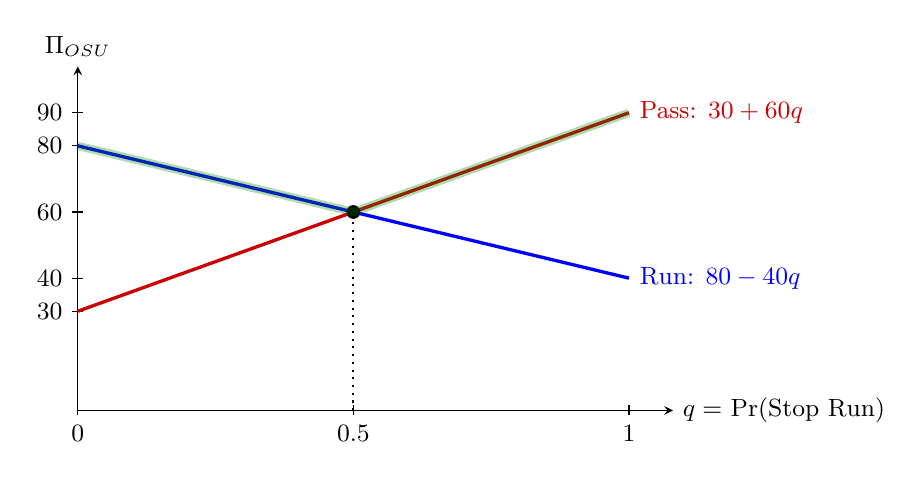
\begin{tikzpicture}[x=7cm, y=0.042cm, >=stealth]
  \draw[->] (0,0) -- (1.08,0) node[right] {\small $q=$ Pr(Stop Run)};
  \draw[->] (0,0) -- (0,104) node[above] {\small $\Pi_{OSU}$};
  \foreach \t in {0,0.5,1}{ \draw (\t,1.5) -- (\t,-1.5) node[below] {\small \t}; }
  \foreach \v in {30,40,60,80,90}{ \draw (0.01,\v) -- (-0.01,\v) node[left] {\small \v}; }
  \onslide<2->{
    \draw[blue, very thick] (0,80) -- (1,40) node[right] {\small Run: $80-40q$};
  }
  \onslide<3->{
    \draw[red!80!black, very thick] (0,30) -- (1,90) node[right] {\small Pass: $30+60q$};
  }
  \onslide<4->{
    \draw[dotted, thick] (0.5,0) -- (0.5,60);
    \fill (0.5,60) circle (2.5pt);
    \draw[line width=3pt, opacity=0.3, green!50!black] (0,80) -- (0.5,60) -- (1,90);
  }
\end{tikzpicture}
\bsk
\raggedright
\only<1-3>{Plot each pure strategy's expected payoff against $q$}%
\only<4>{Best reply $=$ the higher line. \ They cross at $q=$ \underline{\hspace{0.6in}}}
\vspace{-0.2in}
\end{frame}

\begin{frame}{OSU's Best Reply}
$$BR_{OSU}(q)=\begin{cases}
\text{Run} & \text{if } q<\tfrac12 \\[4pt]
\text{\underline{\hspace{1.4in}}} & \text{if } q=\tfrac12 \\[4pt]
\text{Pass} & \text{if } q>\tfrac12
\end{cases}$$
\bsk
\textbf{Fact:} A mix of Run and Pass is a best reply \textbf{only} when Run and Pass tie
\begin{itemize}
    \item Otherwise, shift weight to the better one!
\end{itemize}
\bsk
\textbf{Fact:} When they tie, \textbf{every} mix is a best reply
\vfill
\textbf{In general:} $\sigma_i$ is a best reply $\iff$ every pure strategy it uses is a best reply
\vspace{-0.4in}
\end{frame}

\begin{frame}{Definition: Mixed Strategy}
A \textbf{mixed strategy} $\sigma_i$ is a probability over each of player $i$'s strategies
\bsk
\textbf{Ex:} \ $\sigma_1=\begin{pmatrix} \text{Run} & \text{Pass} \\ p & 1-p\end{pmatrix}$
\qquad
$\sigma_2=\begin{pmatrix} \text{Stop Run} & \text{Stop Pass} \\ q & 1-q\end{pmatrix}$
\bsk
Notation:
\begin{itemize}
    \item $\sigma_i(s_i)$: probability that $\sigma_i$ puts on $s_i$. Rule: $\sum_{s_i} \sigma_i(s_i)=1$
    \begin{itemize}
        \item $\sigma_1(\text{Run})=p$, $\sigma_1(\text{Pass})=1-p$
        \item $\sigma_2(\text{Stop Run})=q$, $\sigma_2(\text{Stop Pass})=1-q$
    \end{itemize}
    \item $\Sigma_i$: set of all mixed strategies of player $i$. So $\sigma_i\in \Sigma_i$
    \item A non-mixed strategy $s_i\in S_i$ is called a a \textbf{pure strategy}
    \begin{itemize}
        \item Pure strategy $=$ mixed strategy with probability 1 on one $s_i$
    \end{itemize}
\end{itemize}
\vfill
\textbf{Assume:} players randomize \textbf{independently} (no correlation)
\vspace{-0.3in}
\end{frame}

\begin{frame}{Expected Payoff of a Mixed Profile}
A mixed strategy profile $\sigma=(\sigma_1,\sigma_2)$ generates a lottery over the \textbf{cells}
\bsk
Probability of cell $s=(s_1,s_2)$: \quad $\sigma(s)=\sigma_1(s_1)\times\sigma_2(s_2)$ \hfill (independence)
\bsk
\textbf{Expected payoff:} weight each cell's payoff by the chance of landing in it
$$\underbrace{\Pi_i(\sigma)\vphantom{\sum_{s}}}_{\text{expected payoff}}\ =\ \sum_{s\in S}\ \underbrace{\sigma(s)\vphantom{\sum_{s}}}_{\text{prob.\ of cell }s}\ \cdot\ \underbrace{\pi_i(s)\vphantom{\sum_{s}}}_{\text{payoff in cell }s}$$
\bsk
Capital $\Pi$: payoff from a mixed profile. Small $\pi$: from a pure profile
\vfill
{\footnotesize Same idea as $U$ vs.\ $u$ in Chapter 5}
\vspace{-0.2in}
\end{frame}

\begin{frame}{Definition: Mixed-Strategy Nash Equilibrium}
In words: every player's mix is a best reply to the other players' mixes
\bsk
A mixed profile $\sigma^*=(\sigma_1^*,\ldots,\sigma_n^*)$ is a \textbf{Nash equilibrium} if, for every player $i$,
$$\underbrace{\Pi_i(\sigma_i^*,\sigma_{-i}^*)}_{\text{payoff from equilibrium mix}}\ \ \ge\ \ \underbrace{\Pi_i(\sigma_i,\sigma_{-i}^*)}_{\text{payoff from any other mix}}\qquad\text{for all }\sigma_i\in\Sigma_i$$
\bsk
Equivalently: $\sigma_i^* \in BR_i(\sigma_{-i}^*)$ for every $i$\\
\only<2->{where $BR_i(\sigma_{-i}^*)=\{\sigma_i^*\in \Sigma_i:\Pi_i(\sigma_i^*,\sigma_{-i}^*)\geq \Pi_i(\sigma_i,\sigma_{-i}^*)\ \ \forall\sigma_i\in\Sigma_i\}$}
\bsk
\onslide<3->{Same as Chapter 2: $s_i^*\in BR_i(s_{-i}^*)$ for every $i$}
\bsk
\vfill
{\footnotesize A pure-strategy NE is still a NE when mixing is allowed (Bonanno p.~211).}
\vspace{-0.2in}
\end{frame}

\begin{frame}{Nash's Theorem}
\begin{block}{Theorem (Nash's 1951 PhD Dissertation at Princeton)}
Every finite game has \textbf{at least one} Nash equilibrium in mixed strategies.\\
{\footnotesize Finite game: finitely many players, each with finitely many strategies.}
\end{block}
\bsk
\begin{itemize}
    \item Matching Pennies: no pure NE, but a mixed one
    \item Run vs. Pass: no pure NE, but a mixed one
\end{itemize}
\bsk
Proof uses ``Kakutani's fixed-point theorem''. (Not covered here.)
\vfill
Recall: We assume players maximize expected utility.
\vspace{-0.4in}
\end{frame}

% ==============================================================
% 6.3 COMPUTING MIXED-STRATEGY NE
% ==============================================================

\begin{frame}[standout]
Finding Mixed Equilibria
\end{frame}

\begin{frame}{The Indifference Principle}
\textbf{Indifference Principle:} If you mix between two strategies in equilibrium, they must have the same expected payoff. (If not, you'd switch to playing the better one for sure!)
\bsk
If $\sigma_i^*$ puts positive probability on both $s_i$ and $s_i'$, then
$$\underbrace{\Pi_i(s_i,\sigma_{-i}^*)}_{\text{payoff from }s_i}\ =\ \underbrace{\Pi_i(s_i',\sigma_{-i}^*)}_{\text{payoff from }s_i'}\ =\ \underbrace{\Pi_i(\sigma^*)}_{\text{equilibrium payoff}}$$
\bsk
\textbf{Implication:}
\begin{enumerate}
    \item If I'm mixing between two strategies in equilibrium, it's because I'm indifferent
    \item Thus, you must be mixing in a way that \textbf{makes me indifferent}
    \item And if you're mixing, I'm also \textbf{making you indifferent}
\end{enumerate}
So, mixed strategy equilibrium $\Rightarrow$ designed to make both players \textbf{indifferent}
\vfill
{\footnotesize Bonanno Theorem 6.3.1}
\vspace{-0.2in}
\end{frame}

\begin{frame}{An Example}
\begin{center}
\begin{matrixgame}[top={L,C,R}, left={T,M,B}, player names={P1,P2}]
  \payoffmatrix{1,0 & 0,1 & 2,-1 \\ 0,2 & 1,0 & 2,-1 \\ -1,0 & -1,0 & 1,3}
\end{matrixgame}
\bsk
\only<1>{$B$ is strictly dominated by $M$}
\only<2>{Then $R$ is strictly dominated by $C$.\\
So, reduce the game to $\{T,M\}\times\{L,C\}$}
\only<3>{Suppose $Pr(L)=q$ and $Pr(C)=1-q$. (We know $Pr(R)=0$)\\When is P1 indifferent between $T$ and $M$?\\
$\Pi_1(\text{T})=q(1)+(1-q)(0)=q$\\
$\Pi_1(\text{M})=q(0)+(1-q)1=1-q$\\
$\Pi_1(T)=\Pi_1(M)\Rightarrow q=1-q\Rightarrow q=1/2$\\
Prediction: P1 plays $q=1/2$}
\only<4>{Suppose $Pr(T)=p$ and $Pr(M)=1-p$. (We know $Pr(B)=0$)\\When is P2 indifferent between $L$ and $C$?\\
$\Pi_2(\text{L})=p(0)+(1-p)(2)=2-2p$\\
$\Pi_2(\text{C})=p(1)+(1-p)0=p$\\
$\Pi_2(T)=\Pi_2(M)\Rightarrow p=2-2p\Rightarrow 3p=2\Rightarrow p=2/3$\\
Prediction: P2 plays $p=2/3$}
    
\end{center}
    
\end{frame}

\begin{frame}{Recipe: Mixed NE in a $2\times 2$}
\begin{enumerate}
    \item Run IDSDS first. Dominated strategies get probability 0
    \bsk
    \item Underline. Note any pure NE
    \bsk
    \item P2 plays $q$, $1-q$. Find the $q$ that makes \textbf{P1} indifferent
    \begin{itemize}
        \item \textbf{Notice:} P2 is making P1 indifferent!
    \end{itemize}
    \bsk
    \item P1 plays $p$, $1-p$. Find the $p$ that makes \textbf{P2} indifferent
    \begin{itemize}
        \item \textbf{Notice:} P1 is making P2 indifferent!
    \end{itemize}
    \bsk
    \item Both strictly between 0 and 1? That's a mixed NE
\end{enumerate}
\vspace{-0.4in}
\end{frame}

\begin{frame}{Solving the Two-Point Game}
\begin{columns}[T]
\begin{column}{0.42\textwidth}
\centering
\begin{matrixgame}[top={Stop Run, Stop Pass}, left={Run, Pass}, player names={Ohio State, Michigan}, w=1.9]
  \payoffmatrix{40,60 & 80,20 \\ 90,10 & 30,70}
\end{matrixgame}
\end{column}
\begin{column}{0.55\textwidth}
\textbf{Step 1:} Michigan's $q$ makes OSU indifferent
\vspace{1.3in}

$q^*=$
\end{column}
\end{columns}
\vfill
\vspace{-0.3in}
\end{frame}

\begin{frame}{Solving the Two-Point Game}
\begin{columns}[T]
\begin{column}{0.42\textwidth}
\centering
\begin{matrixgame}[top={Stop Run, Stop Pass}, left={Run, Pass}, player names={Ohio State, Michigan}, w=1.9]
  \payoffmatrix{40,60 & 80,20 \\ 90,10 & 30,70}
\end{matrixgame}
\end{column}
\begin{column}{0.55\textwidth}
\textbf{Step 2:} OSU's $p$ makes Michigan indifferent
\vspace{1.3in}

$p^*=$
\end{column}
\end{columns}
\bsk
Mixed NE: \hspace{2.5in} OSU scores \underline{\hspace{0.6in}}\% of the time
\vfill
\vspace{-0.3in}
\end{frame}


\begin{frame}{The Unsettling Part of MSNE}
Consider Rock Paper Scissors (RPS) whose MSNE is $\sigma^*=((1/3,1/3,1/3),(1/3,1/3,1/3))$
\begin{itemize}
    \item In the MSNE you're indifferent between Rock, Paper, and Scissors.
    \item But then why do you play $(1/3,1/3,1/3)$?? You have \textbf{no incentive} either way!
\end{itemize}
\bsk
Nash reasoning:
\begin{itemize}
    \item When considering deviating, you assume \textbf{they don't change} their strategy $\sigma_{-i}^*$.
    \item If they're fixed at $(1/3,1/3,1/3)$ then you don't care what you play.
    \item Deviating away from $(1/3,1/3,1/3)$ doesn't help or hurt you.
\end{itemize}
\bsk
``Dynamic'' reasoning:
\begin{itemize}
    \item If you deviate away from $(1/3,1/3,1/3)$ then they'll respond by moving away from $(1/3,1/3,1/3)$ to take advantage of you
    \item ...and then you'd change your strategy, and then so would they...
    \item Only ``stable'' point: Mixed Strategy Nash equilibrium $\sigma^*$
    \begin{itemize}
        \item Caveat: that dynamic process won't \textit{converge} to $\sigma^*$... it'll cycle forever
        \item Stable equilibrium vs. unstable equilibrium. 
    \end{itemize}
\end{itemize}
    
\end{frame}

\begin{frame}{Back to MobLab}
\begin{columns}[T]
\begin{column}{0.48\textwidth}
\centering
\textbf{Round 1}\\[4pt]
\begin{matrixgame}[top={Left, Right}, left={Top, Bottom}, player names={Row, Column}]
  \payoffmatrix{80,40 & 40,80 \\ 40,80 & 80,40}
\end{matrixgame}
\end{column}
\begin{column}{0.48\textwidth}
\centering
\textbf{Round 2}\\[4pt]
\begin{matrixgame}[top={Left, Right}, left={Top, Bottom}, player names={Row, Column}]
  \payoffmatrix{320,40 & 40,80 \\ 40,80 & 80,40}
\end{matrixgame}
\end{column}
\end{columns}
\bsk
Round 1 mixed NE: \vspace{0.35in}

Round 2 mixed NE: \vspace{0.35in}

Only Row's payoff changed. Whose mix changes in the NE??
\end{frame}


\begin{frame}{Back to MobLab}
\vspace{0.2in}
\centering
\renewcommand{\arraystretch}{2}
\begin{tabular}{l|c|c|c|c|}
\cline{2-5}
 & \multicolumn{2}{c|}{\% Rows playing Top} & \multicolumn{2}{c|}{\% Columns playing Left} \\
\cline{2-5}
 & Round 1 & Round 2 & Round 1 & Round 2 \\
\hline
\multicolumn{1}{|l|}{Nash prediction} & 50 & 50 & 50 & 12.5 \\
\hline
\multicolumn{1}{|l|}{Goeree \& Holt (2001)} & $\approx$ 50 & 96 & $\approx$ 50 & 16 \\
\hline
% \multicolumn{1}{|l|}{Our class} & \hspace{0.6in} & \hspace{0.6in} & \hspace{0.6in} & \hspace{0.6in} \\
% \hline
\end{tabular}
\bsk
\raggedright
\textbf{Lab result:} Rows chase the 320. NE says Row's own payoffs shouldn't matter!\\
Columns anticipate it and play Left even less
\vfill
{\footnotesize Not in the book. Source: Goeree \& Holt (2001), ``Ten Little Treasures of Game Theory and Ten Intuitive Contradictions,'' \textit{American Economic Review} 91(5).}
\vspace{-0.2in}
\end{frame}

% ==============================================================
% PURE AND MIXED TOGETHER
% ==============================================================

\begin{frame}[standout]
Pure and Mixed Together
\end{frame}

\begin{frame}{The Sunday Morning Game Revisited}
Alex and Blair, dead phones: Buckeye Donuts or HangOverEasy?
\bsk
\centering
\begin{matrixgame}[top={BuckyDs, HangOE}, left={BuckyDs, HangOE}, player names={Alex, Blair}, br=<2->]
  \payoffmatrix{4,3 & 2,1 \\ 1,2 & 3,4}
\end{matrixgame}
\bsk
\raggedright
Now read the payoffs as \textbf{cardinal} (outcome utilities)
\bsk
\onslide<2->{Pure NE: \underline{\hspace{2in}}}
\bsk
\onslide<3->{Is there also a mixed NE?}
\vspace{-0.3in}
\end{frame}

\begin{frame}{Sunday Morning: The Mixed NE}
\begin{columns}[T]
\begin{column}{0.42\textwidth}
\centering
\begin{matrixgame}[top={BuckyDs, HangOE}, left={BuckyDs, HangOE}, player names={Alex, Blair}]
  \payoffmatrix{4,3 & 2,1 \\ 1,2 & 3,4}
\end{matrixgame}
\end{column}
\begin{column}{0.55\textwidth}
Blair's $q$ makes Alex indifferent:
\vspace{0.6in}

Alex's $p$ makes Blair indifferent:
\vspace{0.6in}
\end{column}
\end{columns}
\bsk
Payoffs at the mixed NE: \ Alex \underline{\hspace{0.5in}} \ Blair \underline{\hspace{0.5in}} \ Better or worse than the pure NE?
\vspace{0.3in}
\end{frame}

\begin{frame}{Indifference Isn't Enough}
\centering
\begin{matrixgame}[top={D, E}, left={A, B, C}, player names={Player 1, Player 2}]
  \payoffmatrix{3,0 & 0,2 \\ 0,2 & 3,0 \\ 2,0 & 2,1}
\end{matrixgame}
\bsk
\raggedright
Try: \ P1 plays $\begin{pmatrix} A & B & C \\ \tfrac12 & \tfrac12 & 0\end{pmatrix}$, \ P2 plays $\begin{pmatrix} D & E \\ \tfrac12 & \tfrac12\end{pmatrix}$
\bsk
P1 indifferent between $A$ and $B$? \ $\Pi_1(A)=$ \hspace{0.6in} $\Pi_1(B)=$
\bsk
\onslide<2->{But $\Pi_1(C)=$ \underline{\hspace{0.5in}} \ So mixing 50-50 over $A$ and $B$ is \textbf{not} a NE!}
\vfill
\onslide<2->{\textbf{Lesson:} Need indifference \textbf{and} no better strategy}
\vspace{-0.3in}
\end{frame}

\begin{frame}{Best Replies With Three Strategies}
\begin{columns}[T]
\begin{column}{0.36\textwidth}
\centering
\scalebox{0.85}{%
\begin{matrixgame}[top={D, E}, left={A, B, C}, player names={Player 1, Player 2}]
  \payoffmatrix{3,0 & 0,2 \\ 0,2 & 3,0 \\ 2,0 & 2,1}
\end{matrixgame}}
\bsk
\raggedright
Pr($D$) $=q_D$\\
Pr($E$) $=q_E=1-q_D$
\bsk
{\color{blue}$\Pi_1(A,q_D)=3q_D$}\\
{\color{red}$\Pi_1(B,q_D)=3(1-q_D)=3-3q_D$}\\
$\Pi_1(C,q_D)=2$
\end{column}
\begin{column}{0.62\textwidth}
\centering
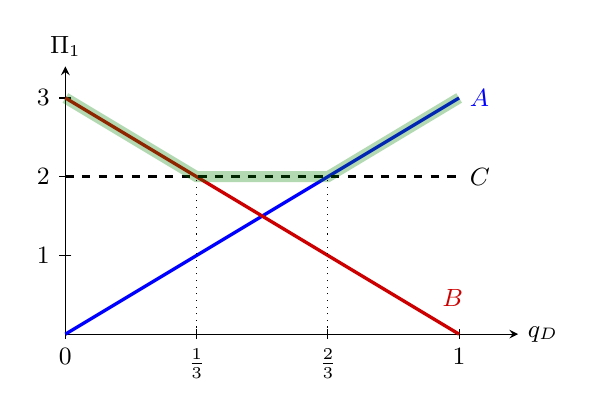
\begin{tikzpicture}[x=5cm, y=1.0cm, >=stealth]
  \draw[->] (0,0) -- (1.15,0) node[right] {\small $q_D$};
  \draw[->] (0,0) -- (0,3.4) node[above] {\small $\Pi_1$};
  \foreach \t/\l in {0/0, 0.3333/\tfrac13, 0.6667/\tfrac23, 1/1}{ \draw (\t,0.06) -- (\t,-0.06) node[below] {\small $\l$}; }
  \foreach \v in {1,2,3}{ \draw (0.015,\v) -- (-0.015,\v) node[left] {\small \v}; }
  \draw[blue, very thick] (0,0) -- (1,3) node[right] {\small $A$};
  \draw[red!80!black, very thick] (0,3) -- (1,0) node[pos=0.93, above right] {\small $B$};
  \draw[black, very thick, dashed] (0,2) -- (1,2) node[right] {\small $C$};
  \onslide<2->{
    \draw[line width=4pt, opacity=0.3, green!50!black] (0,3) -- (0.3333,2) -- (0.6667,2) -- (1,3);
    \draw[dotted] (0.3333,0) -- (0.3333,2);
    \draw[dotted] (0.6667,0) -- (0.6667,2);
  }
\end{tikzpicture}
\end{column}
\end{columns}
\medskip
$BR_1(q_D)$: \hspace{0.3in}
\onslide<2->{$B$ if $q_D<\tfrac13$ \qquad $C$ if $\tfrac13<q_D<\tfrac23$ \qquad $A$ if $q_D>\tfrac23$}
\bsk
\onslide<3->{No pure strategy NE $\Rightarrow$ Must be mixing $\Rightarrow$ Must have $q_D=1/3$ (mix $B$ and $C$) or $q_D=2/3$ (mix $A$ and $C$)}
\end{frame}

\begin{frame}{Best Replies With Three Strategies}
\begin{columns}[T]
\begin{column}{0.5\textwidth}
\centering
\scalebox{0.85}{%
\begin{matrixgame}[top={D, E}, left={A, B, C}, player names={Player 1, Player 2}]
  \payoffmatrix{3,0 & 0,2 \\ 0,2 & 3,0 \\ 2,0 & 2,1}
\end{matrixgame}}
\bsk
\raggedright
Pr($A$) $=p_A$\\
Pr($B$) $=p_B$\\
Pr($C$) $=p_C=1-p_A-p_B$
\bsk
$\Pi_2(D,(p_A,p_B,p_C))=2p_B$\\
$\Pi_2(E,(p_A,p_B,p_C))=2p_A+1p_C=2p_A+(1-p_A-p_B)=1+p_A-p_B$
\end{column}
\begin{column}{0.5\textwidth}
P2 will mix when
\begin{align*}
    2p_B &= 1+p_A-p_B \\
    3p_B &= 1+p_A
\end{align*}
Can't be true if P1 is mixing between $A$ \& $C$ (since $p_B=0$). So P1 must be mixing between $B$ \& $C$ (setting $p_A=0$). Indifference principle:
\begin{align*}
    \Pi_2(D,(p_A,p_B,p_C))&=\Pi_2(E,(p_A,p_B,p_C))\\
    3p_B &= 1+p_A\\
    3p_B &= 1+0 \\
    p_B &= \frac{1}{3}
\end{align*}

\end{column}
\end{columns}
\end{frame}

\begin{frame}{Best Replies With Three Strategies}
\begin{center}
    \begin{matrixgame}[top={D, E}, left={A, B, C}, player names={Player 1, Player 2}]
  \payoffmatrix{3,0 & 0,2 \\ 0,2 & 3,0 \\ 2,0 & 2,1}
\end{matrixgame}
\end{center}
\bsk
Mixed-Strategy Nash equilibrium:
\bsk
P1: $(p_A,p_B,p_C)=(0,1/3,2/3)$ (to make P2 indiff. between D and E)
\bsk
P2: $(q_D,q_E)=(1/3,2/3)$ (to make P1 indiff. between B and C)
\end{frame}

\begin{frame}{What Does Mixing Mean?}
At a mixed NE you're \textbf{indifferent}. So why mix exactly 1/3???
\bsk
Three readings:
\begin{enumerate}
    \item \textbf{Literal randomizing.} Coaches, kickers, poker players
    \bsk
    \item \textbf{Beliefs.} $\sigma_2$ is what P1 \textit{believes} P2 will do
    \begin{itemize}
        \item P2 may not randomize at all. P1 just can't predict them
    \end{itemize}
    \bsk
    \item \textbf{Populations.} 60\% of coaches run, 40\% pass
\end{enumerate}
\vfill
Bonanno calls mixed NE ``conceptually problematic.'' Agree?
\vspace{-0.4in}
\end{frame}

\begin{frame}{Mixing in the Real World}
Lots of situations boil down to ``be unpredictable'':
\bsk
\begin{itemize}
    \item \textbf{Penalty kicks.} Kick left or right? Dive left or right?
    \item \textbf{Tennis serves.} To the forehand or the backhand?
    \item \textbf{Play-calling, pitch selection.} Run/pass. Fastball/curveball
    \item \textbf{Poker.} Bluff with a bad hand, or fold?
    \item \textbf{Inspections.} Tax audits, parking tickets, drug tests, fare checks
    \item \textbf{Security.} LAX randomizes its checkpoints and patrols
\end{itemize}
\bsk
\textbf{Lab/field result:} Pro soccer and tennis players mix close to NE rates
\vfill
{\footnotesize Not in the book. Sources: Walker \& Wooders (2001, \textit{AER}); Chiappori, Levitt \& Groseclose (2002, \textit{AER}); Palacios-Huerta (2003, \textit{REStud}); Pita et al.\ (2008, AAMAS).}
\vspace{-0.2in}
\end{frame}

\begin{frame}{But Those Are More Complicated}
Real versions add:
\begin{itemize}
    \item More than two strategies (left, middle, right)
    \item Repeated play: patterns can be spotted and exploited
    \item Players differ in skill (a left-footed kicker)
    \item Payoffs nobody knows exactly
\end{itemize}
\bsk
Core idea survives: if you're predictable, you get exploited
\vfill
\vspace{-0.4in}
\end{frame}

% ==============================================================
% 6.4 STRICT DOMINANCE AND RATIONALIZABILITY
% ==============================================================

\begin{frame}[standout]
Dominance, Revisited
\end{frame}

\begin{frame}{Remember This One?}
From Chapter 2: $M$ is never a best reply to a \textbf{pure} strategy, but isn't dominated
\bsk
\centering
\begin{matrixgame}[top={L, C, R}, left={U, M, D}, player names={Player 1, Player 2}]
  \payoffmatrix{4,1 & 2,0 & 4,2 \\
                3,2 & 3,1 & 3,0 \\
                0,0 & 4,2 & 0,1}
\end{matrixgame}
\bsk
\raggedright
Suppose P2 plays $\begin{pmatrix} L & C & R \\ 0.4 & 0.6 & 0\end{pmatrix}$
\bsk
$\Pi_1(U)=$ \hspace{0.9in} $\Pi_1(M)=$ \hspace{0.9in} $\Pi_1(D)=$
\bsk
\onslide<2->{$M$ \textbf{is} a best reply, to a \textbf{mixed} strategy!}
\vspace{-0.3in}
\end{frame}

\begin{frame}{Dominated by a Mix}
\centering
\begin{matrixgame}[top={D, E}, left={A, B, C}, player names={Player 1, Player 2}]
  \payoffmatrix{0,1 & 4,0 \\ 1,2 & 1,4 \\ 2,0 & 0,1}
\end{matrixgame}
\bsk
\raggedright
Is $B$ dominated by $A$? By $C$? \vspace{0.3in}

Try the mix $\begin{pmatrix} A & B & C \\ \tfrac13 & 0 & \tfrac23\end{pmatrix}$:
\hspace{0.3in} vs.\ $D$: \hspace{0.8in} vs.\ $E$:
\bsk
\onslide<2->{$B$ is \textbf{strictly dominated by a mixed strategy}\\
So $B$ is never a best reply, to anything P2 might do}
\vspace{-0.3in}
\end{frame}

\begin{frame}{Pearce's Theorem}
\begin{block}{Theorem (Pearce, 1984)}
In a two-player game, $s_i$ is never a best reply to any mixed strategy of the opponent
\begin{center}
$\iff$
\end{center}
$s_i$ is strictly dominated by some mixed strategy of player $i$
\end{block}
\bsk
\begin{itemize}
    \item Fixes Chapter 2's gap: ``never a best reply'' $=$ ``dominated by a mix''
    \item Opponent's mix $=$ my \textbf{belief} about them
    \begin{itemize}
        \item Dominated by a mix $\iff$ irrational under \textbf{every} belief
    \end{itemize}
\end{itemize}
\vfill
{\footnotesize Three or more players: true if beliefs may be correlated (Bonanno \S6.4).}
\vspace{-0.2in}
\end{frame}

\begin{frame}{Cardinal IDSDS}
Same as IDSDS, but also delete strategies dominated by \textbf{mixes}
\begin{itemize}
    \item Survivors are called \textbf{rationalizable} strategies
\end{itemize}
\bsk
\centering
\begin{matrixgame}[top={D, E, F}, left={A, B, C}, player names={Player 1, Player 2}]
  \payoffmatrix{3,4 & 2,1 & 1,2 \\ 0,0 & 1,3 & 4,1 \\ 1,4 & 1,4 & 2,6}
\end{matrixgame}
\bsk
\raggedright
Step 1: \hspace{1.5in} Step 2: \\[0.25in]
Step 3: \hspace{1.5in} Step 4:
\bsk
\textbf{Careful:} needs players to know each other's \textbf{cardinal} payoffs. Realistic?
\vspace{-0.3in}
\end{frame}

% ==============================================================
% WORKED EXAMPLE
% ==============================================================
% Jordan (row): Pay, West, Neil.  CampusParc (col): Patrol West, Patrol Neil
%   Pay:  (1,0) (1,0)    West: (0,2) (4,0)    Neil: (3,0) (0,1)
% Q1 nothing dominated by a pure strategy, for either player
% Q2 Pay dominated by 1/2 West + 1/2 Neil: (1.5, 2) > (1, 1)
% Q3 no pure NE
% Q4 q = Pr(Patrol West): 4(1-q) = 3q -> q = 4/7
%    p = Pr(West):        2p = 1-p    -> p = 1/3
%    NE: Jordan (0, 1/3, 2/3), CampusParc (4/7, 3/7). Payoffs 12/7, 2/3
%    Pay at the NE gives 1 < 12/7, so leaving it out is fine
% Q5 West catch worth 4 to CampusParc: 4p = 1-p -> p = 1/5; q stays 4/7
%    Jordan's payoff unchanged at 12/7; CampusParc's rises to 4/5
% ---------------------------------------------------------------------

\begin{frame}[standout]
Let's Work One Out
\end{frame}

\begin{frame}{Gameday Parking}
Jordan drives to campus for the Michigan game. Three options:
\begin{itemize}
    \item \textbf{Pay} for a gameday lot
    \item Park illegally in a \textbf{West} Campus lot
    \item Park illegally on \textbf{Neil} Ave
\end{itemize}
CampusParc has one tow crew. It can patrol West Campus or Neil Ave
\bsk
\centering
\begin{matrixgame}[top={Patrol West, Patrol Neil}, left={Pay, West, Neil}, player names={Jordan, CampusParc}, w=2.1]
  \payoffmatrix{1,0 & 1,0 \\ 0,2 & 4,0 \\ 3,0 & 0,1}
\end{matrixgame}
\bsk
\raggedright
{\footnotesize Jordan picks the row, CampusParc the column. Payoffs: Jordan, CampusParc. Hypothetical numbers.}
\vspace{-0.2in}
\end{frame}

\begin{frame}{Gameday Parking}
\begin{enumerate}
    \item Is any strategy strictly dominated by a \textbf{pure} strategy? \vspace{0.2in}
    \item Is any strategy strictly dominated by a \textbf{mixed} strategy? Delete it \vspace{0.3in}
    \item Is there a pure-strategy NE? \vspace{0.2in}
    \item Find the mixed NE and both players' expected payoffs. \\
      Check that Jordan really doesn't want to Pay \vspace{0.55in}
    \item CampusParc now earns 4 (not 2) for a tow at West Campus.\\
      Whose mix changes? Does Jordan's payoff change? \vspace{0.3in}
\end{enumerate}
\end{frame}

\begin{frame}{What Have We Learned, Charlie Brown?}
\begin{itemize}
    \item Lottery in a cell? Its expected utility is the payoff
    \item \textbf{Mixed strategy}: a lottery over your own pure strategies
    \item $\Pi_i(\sigma)$: weight each cell's payoff by its probability
    \begin{itemize}
        \item Needs \textbf{cardinal} payoffs. That's why we did Chapter 5
    \end{itemize}
    \item \textbf{Mixed NE}: every mix is a best reply to the others
    \item \textbf{Nash (1951)}: every finite game has one
    \item \textbf{Indifference principle}: my mix makes \textit{you} indifferent
    \begin{itemize}
        \item Necessary, not sufficient. Check unused strategies
    \end{itemize}
    \item \textbf{Pearce}: never a best reply $\iff$ dominated by a mix
\end{itemize}
\vfill
Next: mixing in game trees (behavioral strategies)
\vspace{-0.4in}
\end{frame}

\begin{frame}{Reading \& Practice}
\begin{itemize}
    \item Bonanno, \textit{Game Theory}, Chapter 6
    \begin{itemize}
        \item \S6.1: skim. Lotteries in cells, done formally
        \item \S6.2--6.4: read carefully
    \end{itemize}
    \item Exercises: \S6.5.2 (6.3, 6.4), \S6.5.3 (6.7, 6.8, 6.10), \S6.5.4 (6.12)
    \begin{itemize}
        \item 6.13 and 6.14 are harder. 6.15 (the dog in the river) is a challenge
    \end{itemize}
    \item Solutions in \S6.6. Try them first
\end{itemize}
\vfill
\end{frame}

\end{document}
